\documentclass[11pt,letterpaper]{article}
\usepackage[T1]{fontenc}
\usepackage[utf8]{inputenc}
\usepackage{lmodern}
\usepackage[margin=0.9in]{geometry}
\usepackage{graphicx}
\usepackage{xcolor}
\usepackage{microtype}
\usepackage{listings}
\usepackage[colorlinks=true,linkcolor=blue,urlcolor=blue]{hyperref}
\lstset{
  basicstyle=\ttfamily\footnotesize,
  breaklines=true,breakatwhitespace=false,
  columns=fullflexible,showstringspaces=false,
  frame=single,keepspaces=true,
  postbreak=\mbox{\textcolor{gray}{$\hookrightarrow$}\space}
}
\setlength{\parskip}{0.5em}
\setlength{\parindent}{0pt}
\title{C++23 Syntax and Grammar Reference\\\large Consolidated Source-First LaTeX Collection}
\author{Notoriousjayy Engineering Documentation Library}
\date{November 2026}
\begin{document}
\maketitle
\tableofcontents
\section*{Purpose and provenance}
This is an original learning companion based on a pinned source snapshot, not a
reproduction or normative substitute for the language specification.
The text of all migrated grammar productions is preserved in a machine-readable
JSON source, and rendered for print in the included LaTeX source fragment.
Non-ASCII characters in verbatim grammar renderings are represented as
\texttt{[U+XXXX]} escapes to remain compatible with pdfLaTeX; the data JSON
preserves the source spelling.
\par
\textbf{Specification:} ISO/IEC 14882:2024.
\par
\textbf{Official reference:} \url{https://eel.is/c++draft/gram}
\par
\textbf{Scope limitation:} Declarations, translation phases, contextual grammar, and semantic constraints are not fully captured by standalone grammar productions.
\par
\textbf{Baseline grammar and provenance:} see
\texttt{data/cpp23.json} and
\texttt{data/upstream/cpp23-factory-source.txt}.
The original diagram factory sources are preserved as inert text only.
There is no React or JavaScript application in this collection.

\section*{Railroad diagram}
The curated syntax diagram below is authored in native PlantUML EBNF notation
and uses the repository's existing pinned PlantUML renderer. It is a
verified \emph{illustrative production}, not a claim of visual equivalence to
every rule of the upstream railroad-diagram application.
\begin{center}
\IfFileExists{railroad-samples/png/cpp23.png}{
  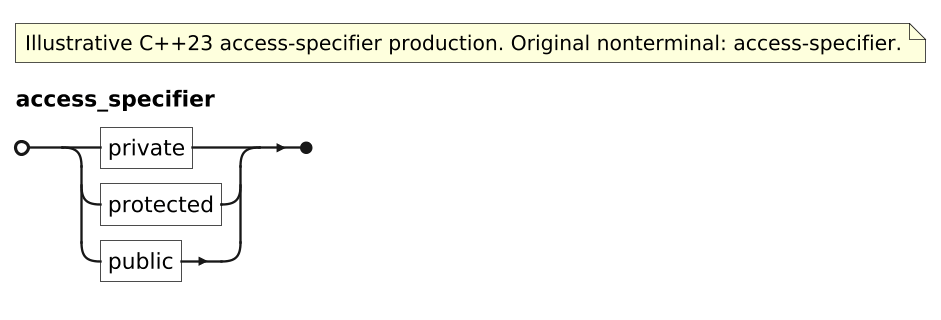
\includegraphics[width=0.85\linewidth]{railroad-samples/png/cpp23.png}
}{
  \fbox{\parbox{0.85\linewidth}{\centering
  Diagram source: \texttt{railroad-samples/cpp23.puml}.
  Render with \texttt{make render-plantuml} using the pinned engine.}}
}
\end{center}
\par
The full text corpus follows. The diagrams do not encode semantic predicates,
contextual constraints or every grammar parsing decision.

% Generated from pinned grammar JSON; printable non-ASCII characters use [U+XXXX] escapes.

\section{keywords}

\noindent\textbf{\texttt{\detokenize{typedef-name}}}\par
\begin{lstlisting}
typedef-name:
    identifier
    simple-template-id
\end{lstlisting}

\noindent\textbf{\texttt{\detokenize{namespace-name}}}\par
\begin{lstlisting}
namespace-name:
    identifier
    namespace-alias
\end{lstlisting}

\noindent\textbf{\texttt{\detokenize{namespace-alias}}}\par
\begin{lstlisting}
namespace-alias:
    identifier
\end{lstlisting}

\noindent\textbf{\texttt{\detokenize{class-name}}}\par
\begin{lstlisting}
class-name:
    identifier
    simple-template-id
\end{lstlisting}

\noindent\textbf{\texttt{\detokenize{enum-name}}}\par
\begin{lstlisting}
enum-name:
    identifier
\end{lstlisting}

\noindent\textbf{\texttt{\detokenize{template-name}}}\par
\begin{lstlisting}
template-name:
    identifier
\end{lstlisting}

\section{lexical}

\noindent\textbf{\texttt{\detokenize{n-char}}}\par
\begin{lstlisting}
n-char:
    any member of the translation character set except } or new-line
\end{lstlisting}

\noindent\textbf{\texttt{\detokenize{n-char-sequence}}}\par
\begin{lstlisting}
n-char-sequence:
    n-char
    n-char-sequence n-char
\end{lstlisting}

\noindent\textbf{\texttt{\detokenize{named-universal-character}}}\par
\begin{lstlisting}
named-universal-character:
    \N{ n-char-sequence }
\end{lstlisting}

\noindent\textbf{\texttt{\detokenize{hex-quad}}}\par
\begin{lstlisting}
hex-quad:
    hexadecimal-digit hexadecimal-digit hexadecimal-digit hexadecimal-digit
\end{lstlisting}

\noindent\textbf{\texttt{\detokenize{simple-hexadecimal-digit-sequence}}}\par
\begin{lstlisting}
simple-hexadecimal-digit-sequence:
    hexadecimal-digit
    simple-hexadecimal-digit-sequence hexadecimal-digit
\end{lstlisting}

\noindent\textbf{\texttt{\detokenize{universal-character-name}}}\par
\begin{lstlisting}
universal-character-name:
    \u hex-quad
    \U hex-quad hex-quad
    \u{ simple-hexadecimal-digit-sequence }
    named-universal-character
\end{lstlisting}

\noindent\textbf{\texttt{\detokenize{preprocessing-token}}}\par
\begin{lstlisting}
preprocessing-token:
    header-name
    import-keyword
    module-keyword
    export-keyword
    identifier
    pp-number
    character-literal
    user-defined-character-literal
    string-literal
    user-defined-string-literal
    preprocessing-op-or-punc
    each non-whitespace character that cannot be one of the above
\end{lstlisting}

\noindent\textbf{\texttt{\detokenize{token}}}\par
\begin{lstlisting}
token:
    identifier
    keyword
    literal
    operator-or-punctuator
\end{lstlisting}

\noindent\textbf{\texttt{\detokenize{header-name}}}\par
\begin{lstlisting}
header-name:
    < h-char-sequence >
    " q-char-sequence "
\end{lstlisting}

\noindent\textbf{\texttt{\detokenize{h-char-sequence}}}\par
\begin{lstlisting}
h-char-sequence:
    h-char
    h-char-sequence h-char
\end{lstlisting}

\noindent\textbf{\texttt{\detokenize{h-char}}}\par
\begin{lstlisting}
h-char:
    any member of the translation character set except new-line and >
\end{lstlisting}

\noindent\textbf{\texttt{\detokenize{q-char-sequence}}}\par
\begin{lstlisting}
q-char-sequence:
    q-char
    q-char-sequence q-char
\end{lstlisting}

\noindent\textbf{\texttt{\detokenize{q-char}}}\par
\begin{lstlisting}
q-char:
    any member of the translation character set except new-line and "
\end{lstlisting}

\noindent\textbf{\texttt{\detokenize{pp-number}}}\par
\begin{lstlisting}
pp-number:
    digit
    . digit
    pp-number identifier-continue
    pp-number ' digit
    pp-number ' nondigit
    pp-number e sign
    pp-number E sign
    pp-number p sign
    pp-number P sign
    pp-number .
\end{lstlisting}

\noindent\textbf{\texttt{\detokenize{identifier}}}\par
\begin{lstlisting}
identifier:
    identifier-start
    identifier identifier-continue
\end{lstlisting}

\noindent\textbf{\texttt{\detokenize{identifier-start}}}\par
\begin{lstlisting}
identifier-start:
    nondigit
    an element of the translation character set with the Unicode property XID_Start
\end{lstlisting}

\noindent\textbf{\texttt{\detokenize{identifier-continue}}}\par
\begin{lstlisting}
identifier-continue:
    digit
    nondigit
    an element of the translation character set with the Unicode property XID_Continue
\end{lstlisting}

\noindent\textbf{\texttt{\detokenize{nondigit}}}\par
\begin{lstlisting}
nondigit: one of
    a b c d e f g h i j k l m
    n o p q r s t u v w x y z
    A B C D E F G H I J K L M
    N O P Q R S T U V W X Y Z _
\end{lstlisting}

\noindent\textbf{\texttt{\detokenize{digit}}}\par
\begin{lstlisting}
digit: one of
    0 1 2 3 4 5 6 7 8 9
\end{lstlisting}

\noindent\textbf{\texttt{\detokenize{keyword}}}\par
\begin{lstlisting}
keyword:
    any identifier listed in Table 5
    import-keyword
    module-keyword
    export-keyword
\end{lstlisting}

\noindent\textbf{\texttt{\detokenize{preprocessing-op-or-punc}}}\par
\begin{lstlisting}
preprocessing-op-or-punc:
    preprocessing-operator
    operator-or-punctuator
\end{lstlisting}

\noindent\textbf{\texttt{\detokenize{preprocessing-operator}}}\par
\begin{lstlisting}
preprocessing-operator: one of
    # ## %: %:%:
\end{lstlisting}

\noindent\textbf{\texttt{\detokenize{operator-or-punctuator}}}\par
\begin{lstlisting}
operator-or-punctuator: one of
    { } [ ] ( )
    <: :> <% %> ; : ...
    ? :: . .* -> ->* ~
    ! + - * / % ^ & |
    = += -= *= /= %= ^= &= |=
    == != < > <= >= <=> && ||
    << >> <<= >>= ++ -- ,
    and or xor not bitand bitor compl
    and_eq or_eq xor_eq not_eq
\end{lstlisting}

\section{literals}

\noindent\textbf{\texttt{\detokenize{literal}}}\par
\begin{lstlisting}
literal:
    integer-literal
    character-literal
    floating-point-literal
    string-literal
    boolean-literal
    pointer-literal
    user-defined-literal
\end{lstlisting}

\noindent\textbf{\texttt{\detokenize{integer-literal}}}\par
\begin{lstlisting}
integer-literal:
    binary-literal integer-suffix_opt
    octal-literal integer-suffix_opt
    decimal-literal integer-suffix_opt
    hexadecimal-literal integer-suffix_opt
\end{lstlisting}

\noindent\textbf{\texttt{\detokenize{binary-literal}}}\par
\begin{lstlisting}
binary-literal:
    0b binary-digit
    0B binary-digit
    binary-literal '_opt binary-digit
\end{lstlisting}

\noindent\textbf{\texttt{\detokenize{octal-literal}}}\par
\begin{lstlisting}
octal-literal:
    0
    octal-literal '_opt octal-digit
\end{lstlisting}

\noindent\textbf{\texttt{\detokenize{decimal-literal}}}\par
\begin{lstlisting}
decimal-literal:
    nonzero-digit
    decimal-literal '_opt digit
\end{lstlisting}

\noindent\textbf{\texttt{\detokenize{hexadecimal-literal}}}\par
\begin{lstlisting}
hexadecimal-literal:
    hexadecimal-prefix hexadecimal-digit-sequence
\end{lstlisting}

\noindent\textbf{\texttt{\detokenize{binary-digit}}}\par
\begin{lstlisting}
binary-digit: one of
    0 1
\end{lstlisting}

\noindent\textbf{\texttt{\detokenize{octal-digit}}}\par
\begin{lstlisting}
octal-digit: one of
    0 1 2 3 4 5 6 7
\end{lstlisting}

\noindent\textbf{\texttt{\detokenize{nonzero-digit}}}\par
\begin{lstlisting}
nonzero-digit: one of
    1 2 3 4 5 6 7 8 9
\end{lstlisting}

\noindent\textbf{\texttt{\detokenize{hexadecimal-prefix}}}\par
\begin{lstlisting}
hexadecimal-prefix: one of
    0x 0X
\end{lstlisting}

\noindent\textbf{\texttt{\detokenize{hexadecimal-digit-sequence}}}\par
\begin{lstlisting}
hexadecimal-digit-sequence:
    hexadecimal-digit
    hexadecimal-digit-sequence '_opt hexadecimal-digit
\end{lstlisting}

\noindent\textbf{\texttt{\detokenize{hexadecimal-digit}}}\par
\begin{lstlisting}
hexadecimal-digit: one of
    0 1 2 3 4 5 6 7 8 9
    a b c d e f
    A B C D E F
\end{lstlisting}

\noindent\textbf{\texttt{\detokenize{integer-suffix}}}\par
\begin{lstlisting}
integer-suffix:
    unsigned-suffix long-suffix_opt
    unsigned-suffix long-long-suffix_opt
    unsigned-suffix size-suffix_opt
    long-suffix unsigned-suffix_opt
    long-long-suffix unsigned-suffix_opt
    size-suffix unsigned-suffix_opt
\end{lstlisting}

\noindent\textbf{\texttt{\detokenize{unsigned-suffix}}}\par
\begin{lstlisting}
unsigned-suffix: one of
    u U
\end{lstlisting}

\noindent\textbf{\texttt{\detokenize{long-suffix}}}\par
\begin{lstlisting}
long-suffix: one of
    l L
\end{lstlisting}

\noindent\textbf{\texttt{\detokenize{long-long-suffix}}}\par
\begin{lstlisting}
long-long-suffix: one of
    ll LL
\end{lstlisting}

\noindent\textbf{\texttt{\detokenize{size-suffix}}}\par
\begin{lstlisting}
size-suffix: one of
    z Z
\end{lstlisting}

\noindent\textbf{\texttt{\detokenize{character-literal}}}\par
\begin{lstlisting}
character-literal:
    encoding-prefix_opt ' c-char-sequence '
\end{lstlisting}

\noindent\textbf{\texttt{\detokenize{encoding-prefix}}}\par
\begin{lstlisting}
encoding-prefix: one of
    u8 u U L
\end{lstlisting}

\noindent\textbf{\texttt{\detokenize{c-char-sequence}}}\par
\begin{lstlisting}
c-char-sequence:
    c-char
    c-char-sequence c-char
\end{lstlisting}

\noindent\textbf{\texttt{\detokenize{c-char}}}\par
\begin{lstlisting}
c-char:
    basic-c-char
    escape-sequence
    universal-character-name
\end{lstlisting}

\noindent\textbf{\texttt{\detokenize{basic-c-char}}}\par
\begin{lstlisting}
basic-c-char:
    any member of the translation character set except ', \, or new-line
\end{lstlisting}

\noindent\textbf{\texttt{\detokenize{escape-sequence}}}\par
\begin{lstlisting}
escape-sequence:
    simple-escape-sequence
    numeric-escape-sequence
    conditional-escape-sequence
\end{lstlisting}

\noindent\textbf{\texttt{\detokenize{simple-escape-sequence}}}\par
\begin{lstlisting}
simple-escape-sequence:
    \ simple-escape-sequence-char
\end{lstlisting}

\noindent\textbf{\texttt{\detokenize{simple-escape-sequence-char}}}\par
\begin{lstlisting}
simple-escape-sequence-char: one of
    ' " ? \ a b f n r t v
\end{lstlisting}

\noindent\textbf{\texttt{\detokenize{numeric-escape-sequence}}}\par
\begin{lstlisting}
numeric-escape-sequence:
    octal-escape-sequence
    hexadecimal-escape-sequence
\end{lstlisting}

\noindent\textbf{\texttt{\detokenize{simple-octal-digit-sequence}}}\par
\begin{lstlisting}
simple-octal-digit-sequence:
    octal-digit
    simple-octal-digit-sequence octal-digit
\end{lstlisting}

\noindent\textbf{\texttt{\detokenize{octal-escape-sequence}}}\par
\begin{lstlisting}
octal-escape-sequence:
    \ octal-digit
    \ octal-digit octal-digit
    \ octal-digit octal-digit octal-digit
    \o{ simple-octal-digit-sequence }
\end{lstlisting}

\noindent\textbf{\texttt{\detokenize{hexadecimal-escape-sequence}}}\par
\begin{lstlisting}
hexadecimal-escape-sequence:
    \x simple-hexadecimal-digit-sequence
    \x{ simple-hexadecimal-digit-sequence }
\end{lstlisting}

\noindent\textbf{\texttt{\detokenize{conditional-escape-sequence}}}\par
\begin{lstlisting}
conditional-escape-sequence:
    \ conditional-escape-sequence-char
\end{lstlisting}

\noindent\textbf{\texttt{\detokenize{conditional-escape-sequence-char}}}\par
\begin{lstlisting}
conditional-escape-sequence-char:
    any member of the basic character set that is not an octal-digit,
    a simple-escape-sequence-char, or the characters N, o, u, U, or x
\end{lstlisting}

\noindent\textbf{\texttt{\detokenize{floating-point-literal}}}\par
\begin{lstlisting}
floating-point-literal:
    decimal-floating-point-literal
    hexadecimal-floating-point-literal
\end{lstlisting}

\noindent\textbf{\texttt{\detokenize{decimal-floating-point-literal}}}\par
\begin{lstlisting}
decimal-floating-point-literal:
    fractional-constant exponent-part_opt floating-point-suffix_opt
    digit-sequence exponent-part floating-point-suffix_opt
\end{lstlisting}

\noindent\textbf{\texttt{\detokenize{hexadecimal-floating-point-literal}}}\par
\begin{lstlisting}
hexadecimal-floating-point-literal:
    hexadecimal-prefix hexadecimal-fractional-constant binary-exponent-part floating-point-suffix_opt
    hexadecimal-prefix hexadecimal-digit-sequence binary-exponent-part floating-point-suffix_opt
\end{lstlisting}

\noindent\textbf{\texttt{\detokenize{fractional-constant}}}\par
\begin{lstlisting}
fractional-constant:
    digit-sequence_opt . digit-sequence
    digit-sequence .
\end{lstlisting}

\noindent\textbf{\texttt{\detokenize{hexadecimal-fractional-constant}}}\par
\begin{lstlisting}
hexadecimal-fractional-constant:
    hexadecimal-digit-sequence_opt . hexadecimal-digit-sequence
    hexadecimal-digit-sequence .
\end{lstlisting}

\noindent\textbf{\texttt{\detokenize{exponent-part}}}\par
\begin{lstlisting}
exponent-part:
    e sign_opt digit-sequence
    E sign_opt digit-sequence
\end{lstlisting}

\noindent\textbf{\texttt{\detokenize{binary-exponent-part}}}\par
\begin{lstlisting}
binary-exponent-part:
    p sign_opt digit-sequence
    P sign_opt digit-sequence
\end{lstlisting}

\noindent\textbf{\texttt{\detokenize{sign}}}\par
\begin{lstlisting}
sign: one of
    + -
\end{lstlisting}

\noindent\textbf{\texttt{\detokenize{digit-sequence}}}\par
\begin{lstlisting}
digit-sequence:
    digit
    digit-sequence '_opt digit
\end{lstlisting}

\noindent\textbf{\texttt{\detokenize{floating-point-suffix}}}\par
\begin{lstlisting}
floating-point-suffix: one of
    f l f16 f32 f64 f128 bf16 F L F16 F32 F64 F128 BF16
\end{lstlisting}

\noindent\textbf{\texttt{\detokenize{string-literal}}}\par
\begin{lstlisting}
string-literal:
    encoding-prefix_opt " s-char-sequence_opt "
    encoding-prefix_opt R raw-string
\end{lstlisting}

\noindent\textbf{\texttt{\detokenize{s-char-sequence}}}\par
\begin{lstlisting}
s-char-sequence:
    s-char
    s-char-sequence s-char
\end{lstlisting}

\noindent\textbf{\texttt{\detokenize{s-char}}}\par
\begin{lstlisting}
s-char:
    basic-s-char
    escape-sequence
    universal-character-name
\end{lstlisting}

\noindent\textbf{\texttt{\detokenize{basic-s-char}}}\par
\begin{lstlisting}
basic-s-char:
    any member of the translation character set except ", \, or new-line
\end{lstlisting}

\noindent\textbf{\texttt{\detokenize{raw-string}}}\par
\begin{lstlisting}
raw-string:
    " d-char-sequence_opt ( r-char-sequence_opt ) d-char-sequence_opt "
\end{lstlisting}

\noindent\textbf{\texttt{\detokenize{r-char-sequence}}}\par
\begin{lstlisting}
r-char-sequence:
    r-char
    r-char-sequence r-char
\end{lstlisting}

\noindent\textbf{\texttt{\detokenize{r-char}}}\par
\begin{lstlisting}
r-char:
    any member of the translation character set, except ) followed by
    the initial d-char-sequence followed by "
\end{lstlisting}

\noindent\textbf{\texttt{\detokenize{d-char-sequence}}}\par
\begin{lstlisting}
d-char-sequence:
    d-char
    d-char-sequence d-char
\end{lstlisting}

\noindent\textbf{\texttt{\detokenize{d-char}}}\par
\begin{lstlisting}
d-char:
    any member of the basic character set except:
    space, (, ), \, horizontal tab, vertical tab, form feed, and new-line
\end{lstlisting}

\noindent\textbf{\texttt{\detokenize{boolean-literal}}}\par
\begin{lstlisting}
boolean-literal:
    false
    true
\end{lstlisting}

\noindent\textbf{\texttt{\detokenize{pointer-literal}}}\par
\begin{lstlisting}
pointer-literal:
    nullptr
\end{lstlisting}

\noindent\textbf{\texttt{\detokenize{user-defined-literal}}}\par
\begin{lstlisting}
user-defined-literal:
    user-defined-integer-literal
    user-defined-floating-point-literal
    user-defined-string-literal
    user-defined-character-literal
\end{lstlisting}

\noindent\textbf{\texttt{\detokenize{user-defined-integer-literal}}}\par
\begin{lstlisting}
user-defined-integer-literal:
    decimal-literal ud-suffix
    octal-literal ud-suffix
    hexadecimal-literal ud-suffix
    binary-literal ud-suffix
\end{lstlisting}

\noindent\textbf{\texttt{\detokenize{user-defined-floating-point-literal}}}\par
\begin{lstlisting}
user-defined-floating-point-literal:
    fractional-constant exponent-part_opt ud-suffix
    digit-sequence exponent-part ud-suffix
    hexadecimal-prefix hexadecimal-fractional-constant binary-exponent-part ud-suffix
    hexadecimal-prefix hexadecimal-digit-sequence binary-exponent-part ud-suffix
\end{lstlisting}

\noindent\textbf{\texttt{\detokenize{user-defined-string-literal}}}\par
\begin{lstlisting}
user-defined-string-literal:
    string-literal ud-suffix
\end{lstlisting}

\noindent\textbf{\texttt{\detokenize{user-defined-character-literal}}}\par
\begin{lstlisting}
user-defined-character-literal:
    character-literal ud-suffix
\end{lstlisting}

\noindent\textbf{\texttt{\detokenize{ud-suffix}}}\par
\begin{lstlisting}
ud-suffix:
    identifier
\end{lstlisting}

\section{basics}

\noindent\textbf{\texttt{\detokenize{translation-unit}}}\par
\begin{lstlisting}
translation-unit:
    declaration-seq_opt
    global-module-fragment_opt module-declaration declaration-seq_opt private-module-fragment_opt
\end{lstlisting}

\section{expressions}

\noindent\textbf{\texttt{\detokenize{primary-expression}}}\par
\begin{lstlisting}
primary-expression:
    literal
    this
    ( expression )
    id-expression
    lambda-expression
    fold-expression
    requires-expression
\end{lstlisting}

\noindent\textbf{\texttt{\detokenize{id-expression}}}\par
\begin{lstlisting}
id-expression:
    unqualified-id
    qualified-id
\end{lstlisting}

\noindent\textbf{\texttt{\detokenize{unqualified-id}}}\par
\begin{lstlisting}
unqualified-id:
    identifier
    operator-function-id
    conversion-function-id
    literal-operator-id
    ~ type-name
    ~ decltype-specifier
    template-id
\end{lstlisting}

\noindent\textbf{\texttt{\detokenize{qualified-id}}}\par
\begin{lstlisting}
qualified-id:
    nested-name-specifier template_opt unqualified-id
\end{lstlisting}

\noindent\textbf{\texttt{\detokenize{nested-name-specifier}}}\par
\begin{lstlisting}
nested-name-specifier:
    ::
    type-name ::
    namespace-name ::
    decltype-specifier ::
    nested-name-specifier identifier ::
    nested-name-specifier template_opt simple-template-id ::
\end{lstlisting}

\noindent\textbf{\texttt{\detokenize{lambda-expression}}}\par
\begin{lstlisting}
lambda-expression:
    lambda-introducer attribute-specifier-seq_opt lambda-declarator compound-statement
    lambda-introducer < template-parameter-list > requires-clause_opt attribute-specifier-seq_opt
        lambda-declarator compound-statement
\end{lstlisting}

\noindent\textbf{\texttt{\detokenize{lambda-introducer}}}\par
\begin{lstlisting}
lambda-introducer:
    [ lambda-capture_opt ]
\end{lstlisting}

\noindent\textbf{\texttt{\detokenize{lambda-declarator}}}\par
\begin{lstlisting}
lambda-declarator:
    lambda-specifier-seq noexcept-specifier_opt attribute-specifier-seq_opt trailing-return-type_opt
    noexcept-specifier attribute-specifier-seq_opt trailing-return-type_opt
    trailing-return-type_opt
    ( parameter-declaration-clause ) lambda-specifier-seq_opt noexcept-specifier_opt
        attribute-specifier-seq_opt trailing-return-type_opt requires-clause_opt
\end{lstlisting}

\noindent\textbf{\texttt{\detokenize{lambda-specifier}}}\par
\begin{lstlisting}
lambda-specifier:
    consteval
    constexpr
    mutable
    static
\end{lstlisting}

\noindent\textbf{\texttt{\detokenize{lambda-specifier-seq}}}\par
\begin{lstlisting}
lambda-specifier-seq:
    lambda-specifier
    lambda-specifier lambda-specifier-seq
\end{lstlisting}

\noindent\textbf{\texttt{\detokenize{lambda-capture}}}\par
\begin{lstlisting}
lambda-capture:
    capture-default
    capture-list
    capture-default , capture-list
\end{lstlisting}

\noindent\textbf{\texttt{\detokenize{capture-default}}}\par
\begin{lstlisting}
capture-default:
    &
    =
\end{lstlisting}

\noindent\textbf{\texttt{\detokenize{capture-list}}}\par
\begin{lstlisting}
capture-list:
    capture
    capture-list , capture
\end{lstlisting}

\noindent\textbf{\texttt{\detokenize{capture}}}\par
\begin{lstlisting}
capture:
    simple-capture
    init-capture
\end{lstlisting}

\noindent\textbf{\texttt{\detokenize{simple-capture}}}\par
\begin{lstlisting}
simple-capture:
    identifier ..._opt
    & identifier ..._opt
    this
    * this
\end{lstlisting}

\noindent\textbf{\texttt{\detokenize{init-capture}}}\par
\begin{lstlisting}
init-capture:
    ..._opt identifier initializer
    & ..._opt identifier initializer
\end{lstlisting}

\noindent\textbf{\texttt{\detokenize{fold-expression}}}\par
\begin{lstlisting}
fold-expression:
    ( cast-expression fold-operator ... )
    ( ... fold-operator cast-expression )
    ( cast-expression fold-operator ... fold-operator cast-expression )
\end{lstlisting}

\noindent\textbf{\texttt{\detokenize{fold-operator}}}\par
\begin{lstlisting}
fold-operator: one of
    + - * / % ^ & | << >>
    += -= *= /= %= ^= &= |= <<= >>= =
    == != < > <= >= && || , .* ->*
\end{lstlisting}

\noindent\textbf{\texttt{\detokenize{requires-expression}}}\par
\begin{lstlisting}
requires-expression:
    requires requirement-parameter-list_opt requirement-body
\end{lstlisting}

\noindent\textbf{\texttt{\detokenize{requirement-parameter-list}}}\par
\begin{lstlisting}
requirement-parameter-list:
    ( parameter-declaration-clause )
\end{lstlisting}

\noindent\textbf{\texttt{\detokenize{requirement-body}}}\par
\begin{lstlisting}
requirement-body:
    { requirement-seq }
\end{lstlisting}

\noindent\textbf{\texttt{\detokenize{requirement-seq}}}\par
\begin{lstlisting}
requirement-seq:
    requirement
    requirement requirement-seq
\end{lstlisting}

\noindent\textbf{\texttt{\detokenize{requirement}}}\par
\begin{lstlisting}
requirement:
    simple-requirement
    type-requirement
    compound-requirement
    nested-requirement
\end{lstlisting}

\noindent\textbf{\texttt{\detokenize{simple-requirement}}}\par
\begin{lstlisting}
simple-requirement:
    expression ;
\end{lstlisting}

\noindent\textbf{\texttt{\detokenize{type-requirement}}}\par
\begin{lstlisting}
type-requirement:
    typename nested-name-specifier_opt type-name ;
\end{lstlisting}

\noindent\textbf{\texttt{\detokenize{compound-requirement}}}\par
\begin{lstlisting}
compound-requirement:
    { expression } noexcept_opt return-type-requirement_opt ;
\end{lstlisting}

\noindent\textbf{\texttt{\detokenize{return-type-requirement}}}\par
\begin{lstlisting}
return-type-requirement:
    -> type-constraint
\end{lstlisting}

\noindent\textbf{\texttt{\detokenize{nested-requirement}}}\par
\begin{lstlisting}
nested-requirement:
    requires constraint-expression ;
\end{lstlisting}

\noindent\textbf{\texttt{\detokenize{postfix-expression}}}\par
\begin{lstlisting}
postfix-expression:
    primary-expression
    postfix-expression [ expression-list_opt ]
    postfix-expression ( expression-list_opt )
    simple-type-specifier ( expression-list_opt )
    typename-specifier ( expression-list_opt )
    simple-type-specifier braced-init-list
    typename-specifier braced-init-list
    postfix-expression . template_opt id-expression
    postfix-expression -> template_opt id-expression
    postfix-expression ++
    postfix-expression --
    dynamic_cast < type-id > ( expression )
    static_cast < type-id > ( expression )
    reinterpret_cast < type-id > ( expression )
    const_cast < type-id > ( expression )
    typeid ( expression )
    typeid ( type-id )
\end{lstlisting}

\noindent\textbf{\texttt{\detokenize{expression-list}}}\par
\begin{lstlisting}
expression-list:
    initializer-list
\end{lstlisting}

\noindent\textbf{\texttt{\detokenize{unary-expression}}}\par
\begin{lstlisting}
unary-expression:
    postfix-expression
    unary-operator cast-expression
    ++ cast-expression
    -- cast-expression
    await-expression
    sizeof unary-expression
    sizeof ( type-id )
    sizeof ... ( identifier )
    alignof ( type-id )
    noexcept-expression
    new-expression
    delete-expression
\end{lstlisting}

\noindent\textbf{\texttt{\detokenize{unary-operator}}}\par
\begin{lstlisting}
unary-operator: one of
    * & + - ! ~
\end{lstlisting}

\noindent\textbf{\texttt{\detokenize{await-expression}}}\par
\begin{lstlisting}
await-expression:
    co_await cast-expression
\end{lstlisting}

\noindent\textbf{\texttt{\detokenize{noexcept-expression}}}\par
\begin{lstlisting}
noexcept-expression:
    noexcept ( expression )
\end{lstlisting}

\noindent\textbf{\texttt{\detokenize{new-expression}}}\par
\begin{lstlisting}
new-expression:
    ::_opt new new-placement_opt new-type-id new-initializer_opt
    ::_opt new new-placement_opt ( type-id ) new-initializer_opt
\end{lstlisting}

\noindent\textbf{\texttt{\detokenize{new-placement}}}\par
\begin{lstlisting}
new-placement:
    ( expression-list )
\end{lstlisting}

\noindent\textbf{\texttt{\detokenize{new-type-id}}}\par
\begin{lstlisting}
new-type-id:
    type-specifier-seq new-declarator_opt
\end{lstlisting}

\noindent\textbf{\texttt{\detokenize{new-declarator}}}\par
\begin{lstlisting}
new-declarator:
    ptr-operator new-declarator_opt
    noptr-new-declarator
\end{lstlisting}

\noindent\textbf{\texttt{\detokenize{noptr-new-declarator}}}\par
\begin{lstlisting}
noptr-new-declarator:
    [ expression_opt ] attribute-specifier-seq_opt
    noptr-new-declarator [ constant-expression ] attribute-specifier-seq_opt
\end{lstlisting}

\noindent\textbf{\texttt{\detokenize{new-initializer}}}\par
\begin{lstlisting}
new-initializer:
    ( expression-list_opt )
    braced-init-list
\end{lstlisting}

\noindent\textbf{\texttt{\detokenize{delete-expression}}}\par
\begin{lstlisting}
delete-expression:
    ::_opt delete cast-expression
    ::_opt delete [ ] cast-expression
\end{lstlisting}

\noindent\textbf{\texttt{\detokenize{cast-expression}}}\par
\begin{lstlisting}
cast-expression:
    unary-expression
    ( type-id ) cast-expression
\end{lstlisting}

\noindent\textbf{\texttt{\detokenize{pm-expression}}}\par
\begin{lstlisting}
pm-expression:
    cast-expression
    pm-expression .* cast-expression
    pm-expression ->* cast-expression
\end{lstlisting}

\noindent\textbf{\texttt{\detokenize{multiplicative-expression}}}\par
\begin{lstlisting}
multiplicative-expression:
    pm-expression
    multiplicative-expression * pm-expression
    multiplicative-expression / pm-expression
    multiplicative-expression % pm-expression
\end{lstlisting}

\noindent\textbf{\texttt{\detokenize{additive-expression}}}\par
\begin{lstlisting}
additive-expression:
    multiplicative-expression
    additive-expression + multiplicative-expression
    additive-expression - multiplicative-expression
\end{lstlisting}

\noindent\textbf{\texttt{\detokenize{shift-expression}}}\par
\begin{lstlisting}
shift-expression:
    additive-expression
    shift-expression << additive-expression
    shift-expression >> additive-expression
\end{lstlisting}

\noindent\textbf{\texttt{\detokenize{compare-expression}}}\par
\begin{lstlisting}
compare-expression:
    shift-expression
    compare-expression <=> shift-expression
\end{lstlisting}

\noindent\textbf{\texttt{\detokenize{relational-expression}}}\par
\begin{lstlisting}
relational-expression:
    compare-expression
    relational-expression < compare-expression
    relational-expression > compare-expression
    relational-expression <= compare-expression
    relational-expression >= compare-expression
\end{lstlisting}

\noindent\textbf{\texttt{\detokenize{equality-expression}}}\par
\begin{lstlisting}
equality-expression:
    relational-expression
    equality-expression == relational-expression
    equality-expression != relational-expression
\end{lstlisting}

\noindent\textbf{\texttt{\detokenize{and-expression}}}\par
\begin{lstlisting}
and-expression:
    equality-expression
    and-expression & equality-expression
\end{lstlisting}

\noindent\textbf{\texttt{\detokenize{exclusive-or-expression}}}\par
\begin{lstlisting}
exclusive-or-expression:
    and-expression
    exclusive-or-expression ^ and-expression
\end{lstlisting}

\noindent\textbf{\texttt{\detokenize{inclusive-or-expression}}}\par
\begin{lstlisting}
inclusive-or-expression:
    exclusive-or-expression
    inclusive-or-expression | exclusive-or-expression
\end{lstlisting}

\noindent\textbf{\texttt{\detokenize{logical-and-expression}}}\par
\begin{lstlisting}
logical-and-expression:
    inclusive-or-expression
    logical-and-expression && inclusive-or-expression
\end{lstlisting}

\noindent\textbf{\texttt{\detokenize{logical-or-expression}}}\par
\begin{lstlisting}
logical-or-expression:
    logical-and-expression
    logical-or-expression || logical-and-expression
\end{lstlisting}

\noindent\textbf{\texttt{\detokenize{conditional-expression}}}\par
\begin{lstlisting}
conditional-expression:
    logical-or-expression
    logical-or-expression ? expression : assignment-expression
\end{lstlisting}

\noindent\textbf{\texttt{\detokenize{yield-expression}}}\par
\begin{lstlisting}
yield-expression:
    co_yield assignment-expression
    co_yield braced-init-list
\end{lstlisting}

\noindent\textbf{\texttt{\detokenize{throw-expression}}}\par
\begin{lstlisting}
throw-expression:
    throw assignment-expression_opt
\end{lstlisting}

\noindent\textbf{\texttt{\detokenize{assignment-expression}}}\par
\begin{lstlisting}
assignment-expression:
    conditional-expression
    yield-expression
    throw-expression
    logical-or-expression assignment-operator initializer-clause
\end{lstlisting}

\noindent\textbf{\texttt{\detokenize{assignment-operator}}}\par
\begin{lstlisting}
assignment-operator: one of
    = *= /= %= += -= >>= <<= &= ^= |=
\end{lstlisting}

\noindent\textbf{\texttt{\detokenize{expression}}}\par
\begin{lstlisting}
expression:
    assignment-expression
    expression , assignment-expression
\end{lstlisting}

\noindent\textbf{\texttt{\detokenize{constant-expression}}}\par
\begin{lstlisting}
constant-expression:
    conditional-expression
\end{lstlisting}

\section{statements}

\noindent\textbf{\texttt{\detokenize{statement}}}\par
\begin{lstlisting}
statement:
    labeled-statement
    attribute-specifier-seq_opt expression-statement
    attribute-specifier-seq_opt compound-statement
    attribute-specifier-seq_opt selection-statement
    attribute-specifier-seq_opt iteration-statement
    attribute-specifier-seq_opt jump-statement
    declaration-statement
    attribute-specifier-seq_opt try-block
\end{lstlisting}

\noindent\textbf{\texttt{\detokenize{init-statement}}}\par
\begin{lstlisting}
init-statement:
    expression-statement
    simple-declaration
    alias-declaration
\end{lstlisting}

\noindent\textbf{\texttt{\detokenize{condition}}}\par
\begin{lstlisting}
condition:
    expression
    attribute-specifier-seq_opt decl-specifier-seq declarator brace-or-equal-initializer
\end{lstlisting}

\noindent\textbf{\texttt{\detokenize{label}}}\par
\begin{lstlisting}
label:
    attribute-specifier-seq_opt identifier :
    attribute-specifier-seq_opt case constant-expression :
    attribute-specifier-seq_opt default :
\end{lstlisting}

\noindent\textbf{\texttt{\detokenize{labeled-statement}}}\par
\begin{lstlisting}
labeled-statement:
    label statement
\end{lstlisting}

\noindent\textbf{\texttt{\detokenize{expression-statement}}}\par
\begin{lstlisting}
expression-statement:
    expression_opt ;
\end{lstlisting}

\noindent\textbf{\texttt{\detokenize{compound-statement}}}\par
\begin{lstlisting}
compound-statement:
    { statement-seq_opt label-seq_opt }
\end{lstlisting}

\noindent\textbf{\texttt{\detokenize{statement-seq}}}\par
\begin{lstlisting}
statement-seq:
    statement
    statement-seq statement
\end{lstlisting}

\noindent\textbf{\texttt{\detokenize{label-seq}}}\par
\begin{lstlisting}
label-seq:
    label
    label-seq label
\end{lstlisting}

\noindent\textbf{\texttt{\detokenize{selection-statement}}}\par
\begin{lstlisting}
selection-statement:
    if constexpr_opt ( init-statement_opt condition ) statement
    if constexpr_opt ( init-statement_opt condition ) statement else statement
    if !_opt consteval compound-statement
    if !_opt consteval compound-statement else statement
    switch ( init-statement_opt condition ) statement
\end{lstlisting}

\noindent\textbf{\texttt{\detokenize{iteration-statement}}}\par
\begin{lstlisting}
iteration-statement:
    while ( condition ) statement
    do statement while ( expression ) ;
    for ( init-statement condition_opt ; expression_opt ) statement
    for ( init-statement_opt for-range-declaration : for-range-initializer ) statement
\end{lstlisting}

\noindent\textbf{\texttt{\detokenize{for-range-declaration}}}\par
\begin{lstlisting}
for-range-declaration:
    attribute-specifier-seq_opt decl-specifier-seq declarator
    attribute-specifier-seq_opt decl-specifier-seq ref-qualifier_opt [ identifier-list ]
\end{lstlisting}

\noindent\textbf{\texttt{\detokenize{for-range-initializer}}}\par
\begin{lstlisting}
for-range-initializer:
    expr-or-braced-init-list
\end{lstlisting}

\noindent\textbf{\texttt{\detokenize{jump-statement}}}\par
\begin{lstlisting}
jump-statement:
    break ;
    continue ;
    return expr-or-braced-init-list_opt ;
    coroutine-return-statement
    goto identifier ;
\end{lstlisting}

\noindent\textbf{\texttt{\detokenize{coroutine-return-statement}}}\par
\begin{lstlisting}
coroutine-return-statement:
    co_return expr-or-braced-init-list_opt ;
\end{lstlisting}

\noindent\textbf{\texttt{\detokenize{declaration-statement}}}\par
\begin{lstlisting}
declaration-statement:
    block-declaration
\end{lstlisting}

\section{declarations}

\noindent\textbf{\texttt{\detokenize{declaration-seq}}}\par
\begin{lstlisting}
declaration-seq:
    declaration
    declaration-seq declaration
\end{lstlisting}

\noindent\textbf{\texttt{\detokenize{declaration}}}\par
\begin{lstlisting}
declaration:
    name-declaration
    special-declaration
\end{lstlisting}

\noindent\textbf{\texttt{\detokenize{name-declaration}}}\par
\begin{lstlisting}
name-declaration:
    block-declaration
    nodeclspec-function-declaration
    function-definition
    template-declaration
    deduction-guide
    linkage-specification
    namespace-definition
    empty-declaration
    attribute-declaration
    module-import-declaration
\end{lstlisting}

\noindent\textbf{\texttt{\detokenize{special-declaration}}}\par
\begin{lstlisting}
special-declaration:
    explicit-instantiation
    explicit-specialization
    export-declaration
\end{lstlisting}

\noindent\textbf{\texttt{\detokenize{block-declaration}}}\par
\begin{lstlisting}
block-declaration:
    simple-declaration
    asm-declaration
    namespace-alias-definition
    using-declaration
    using-enum-declaration
    using-directive
    static_assert-declaration
    alias-declaration
    opaque-enum-declaration
\end{lstlisting}

\noindent\textbf{\texttt{\detokenize{nodeclspec-function-declaration}}}\par
\begin{lstlisting}
nodeclspec-function-declaration:
    attribute-specifier-seq_opt declarator ;
\end{lstlisting}

\noindent\textbf{\texttt{\detokenize{alias-declaration}}}\par
\begin{lstlisting}
alias-declaration:
    using identifier attribute-specifier-seq_opt = defining-type-id ;
\end{lstlisting}

\noindent\textbf{\texttt{\detokenize{simple-declaration}}}\par
\begin{lstlisting}
simple-declaration:
    decl-specifier-seq init-declarator-list_opt ;
    attribute-specifier-seq decl-specifier-seq init-declarator-list ;
    attribute-specifier-seq_opt decl-specifier-seq ref-qualifier_opt [ identifier-list ] initializer ;
\end{lstlisting}

\noindent\textbf{\texttt{\detokenize{static_assert-declaration}}}\par
\begin{lstlisting}
static_assert-declaration:
    static_assert ( constant-expression ) ;
    static_assert ( constant-expression , string-literal ) ;
\end{lstlisting}

\noindent\textbf{\texttt{\detokenize{empty-declaration}}}\par
\begin{lstlisting}
empty-declaration:
    ;
\end{lstlisting}

\noindent\textbf{\texttt{\detokenize{attribute-declaration}}}\par
\begin{lstlisting}
attribute-declaration:
    attribute-specifier-seq ;
\end{lstlisting}

\noindent\textbf{\texttt{\detokenize{decl-specifier}}}\par
\begin{lstlisting}
decl-specifier:
    storage-class-specifier
    defining-type-specifier
    function-specifier
    friend
    typedef
    constexpr
    consteval
    constinit
    inline
\end{lstlisting}

\noindent\textbf{\texttt{\detokenize{decl-specifier-seq}}}\par
\begin{lstlisting}
decl-specifier-seq:
    decl-specifier attribute-specifier-seq_opt
    decl-specifier decl-specifier-seq
\end{lstlisting}

\noindent\textbf{\texttt{\detokenize{storage-class-specifier}}}\par
\begin{lstlisting}
storage-class-specifier:
    static
    thread_local
    extern
    mutable
\end{lstlisting}

\noindent\textbf{\texttt{\detokenize{function-specifier}}}\par
\begin{lstlisting}
function-specifier:
    virtual
    explicit-specifier
\end{lstlisting}

\noindent\textbf{\texttt{\detokenize{explicit-specifier}}}\par
\begin{lstlisting}
explicit-specifier:
    explicit ( constant-expression )
    explicit
\end{lstlisting}

\noindent\textbf{\texttt{\detokenize{type-specifier}}}\par
\begin{lstlisting}
type-specifier:
    simple-type-specifier
    elaborated-type-specifier
    typename-specifier
    cv-qualifier
\end{lstlisting}

\noindent\textbf{\texttt{\detokenize{type-specifier-seq}}}\par
\begin{lstlisting}
type-specifier-seq:
    type-specifier attribute-specifier-seq_opt
    type-specifier type-specifier-seq
\end{lstlisting}

\noindent\textbf{\texttt{\detokenize{defining-type-specifier}}}\par
\begin{lstlisting}
defining-type-specifier:
    type-specifier
    class-specifier
    enum-specifier
\end{lstlisting}

\noindent\textbf{\texttt{\detokenize{defining-type-specifier-seq}}}\par
\begin{lstlisting}
defining-type-specifier-seq:
    defining-type-specifier attribute-specifier-seq_opt
    defining-type-specifier defining-type-specifier-seq
\end{lstlisting}

\noindent\textbf{\texttt{\detokenize{simple-type-specifier}}}\par
\begin{lstlisting}
simple-type-specifier:
    nested-name-specifier_opt type-name
    nested-name-specifier template simple-template-id
    decltype-specifier
    placeholder-type-specifier
    nested-name-specifier_opt template-name
    char
    char8_t
    char16_t
    char32_t
    wchar_t
    bool
    short
    int
    long
    signed
    unsigned
    float
    double
    void
\end{lstlisting}

\noindent\textbf{\texttt{\detokenize{type-name}}}\par
\begin{lstlisting}
type-name:
    class-name
    enum-name
    typedef-name
\end{lstlisting}

\noindent\textbf{\texttt{\detokenize{elaborated-type-specifier}}}\par
\begin{lstlisting}
elaborated-type-specifier:
    class-key attribute-specifier-seq_opt nested-name-specifier_opt identifier
    class-key simple-template-id
    class-key nested-name-specifier template_opt simple-template-id
    enum nested-name-specifier_opt identifier
\end{lstlisting}

\noindent\textbf{\texttt{\detokenize{decltype-specifier}}}\par
\begin{lstlisting}
decltype-specifier:
    decltype ( expression )
\end{lstlisting}

\noindent\textbf{\texttt{\detokenize{placeholder-type-specifier}}}\par
\begin{lstlisting}
placeholder-type-specifier:
    type-constraint_opt auto
    type-constraint_opt decltype ( auto )
\end{lstlisting}

\noindent\textbf{\texttt{\detokenize{init-declarator-list}}}\par
\begin{lstlisting}
init-declarator-list:
    init-declarator
    init-declarator-list , init-declarator
\end{lstlisting}

\noindent\textbf{\texttt{\detokenize{init-declarator}}}\par
\begin{lstlisting}
init-declarator:
    declarator initializer_opt
    declarator requires-clause
\end{lstlisting}

\noindent\textbf{\texttt{\detokenize{declarator}}}\par
\begin{lstlisting}
declarator:
    ptr-declarator
    noptr-declarator parameters-and-qualifiers trailing-return-type
\end{lstlisting}

\noindent\textbf{\texttt{\detokenize{ptr-declarator}}}\par
\begin{lstlisting}
ptr-declarator:
    noptr-declarator
    ptr-operator ptr-declarator
\end{lstlisting}

\noindent\textbf{\texttt{\detokenize{noptr-declarator}}}\par
\begin{lstlisting}
noptr-declarator:
    declarator-id attribute-specifier-seq_opt
    noptr-declarator parameters-and-qualifiers
    noptr-declarator [ constant-expression_opt ] attribute-specifier-seq_opt
    ( ptr-declarator )
\end{lstlisting}

\noindent\textbf{\texttt{\detokenize{parameters-and-qualifiers}}}\par
\begin{lstlisting}
parameters-and-qualifiers:
    ( parameter-declaration-clause ) cv-qualifier-seq_opt
        ref-qualifier_opt noexcept-specifier_opt attribute-specifier-seq_opt
\end{lstlisting}

\noindent\textbf{\texttt{\detokenize{trailing-return-type}}}\par
\begin{lstlisting}
trailing-return-type:
    -> type-id
\end{lstlisting}

\noindent\textbf{\texttt{\detokenize{ptr-operator}}}\par
\begin{lstlisting}
ptr-operator:
    * attribute-specifier-seq_opt cv-qualifier-seq_opt
    & attribute-specifier-seq_opt
    && attribute-specifier-seq_opt
    nested-name-specifier * attribute-specifier-seq_opt cv-qualifier-seq_opt
\end{lstlisting}

\noindent\textbf{\texttt{\detokenize{cv-qualifier-seq}}}\par
\begin{lstlisting}
cv-qualifier-seq:
    cv-qualifier cv-qualifier-seq_opt
\end{lstlisting}

\noindent\textbf{\texttt{\detokenize{cv-qualifier}}}\par
\begin{lstlisting}
cv-qualifier:
    const
    volatile
\end{lstlisting}

\noindent\textbf{\texttt{\detokenize{ref-qualifier}}}\par
\begin{lstlisting}
ref-qualifier:
    &
    &&
\end{lstlisting}

\noindent\textbf{\texttt{\detokenize{declarator-id}}}\par
\begin{lstlisting}
declarator-id:
    ..._opt id-expression
\end{lstlisting}

\noindent\textbf{\texttt{\detokenize{type-id}}}\par
\begin{lstlisting}
type-id:
    type-specifier-seq abstract-declarator_opt
\end{lstlisting}

\noindent\textbf{\texttt{\detokenize{defining-type-id}}}\par
\begin{lstlisting}
defining-type-id:
    defining-type-specifier-seq abstract-declarator_opt
\end{lstlisting}

\noindent\textbf{\texttt{\detokenize{abstract-declarator}}}\par
\begin{lstlisting}
abstract-declarator:
    ptr-abstract-declarator
    noptr-abstract-declarator_opt parameters-and-qualifiers trailing-return-type
    abstract-pack-declarator
\end{lstlisting}

\noindent\textbf{\texttt{\detokenize{ptr-abstract-declarator}}}\par
\begin{lstlisting}
ptr-abstract-declarator:
    noptr-abstract-declarator
    ptr-operator ptr-abstract-declarator_opt
\end{lstlisting}

\noindent\textbf{\texttt{\detokenize{noptr-abstract-declarator}}}\par
\begin{lstlisting}
noptr-abstract-declarator:
    noptr-abstract-declarator_opt parameters-and-qualifiers
    noptr-abstract-declarator_opt [ constant-expression_opt ] attribute-specifier-seq_opt
    ( ptr-abstract-declarator )
\end{lstlisting}

\noindent\textbf{\texttt{\detokenize{abstract-pack-declarator}}}\par
\begin{lstlisting}
abstract-pack-declarator:
    noptr-abstract-pack-declarator
    ptr-operator abstract-pack-declarator
\end{lstlisting}

\noindent\textbf{\texttt{\detokenize{noptr-abstract-pack-declarator}}}\par
\begin{lstlisting}
noptr-abstract-pack-declarator:
    noptr-abstract-pack-declarator parameters-and-qualifiers
    noptr-abstract-pack-declarator [ constant-expression_opt ] attribute-specifier-seq_opt
    ...
\end{lstlisting}

\noindent\textbf{\texttt{\detokenize{parameter-declaration-clause}}}\par
\begin{lstlisting}
parameter-declaration-clause:
    parameter-declaration-list_opt ..._opt
    parameter-declaration-list , ...
\end{lstlisting}

\noindent\textbf{\texttt{\detokenize{parameter-declaration-list}}}\par
\begin{lstlisting}
parameter-declaration-list:
    parameter-declaration
    parameter-declaration-list , parameter-declaration
\end{lstlisting}

\noindent\textbf{\texttt{\detokenize{parameter-declaration}}}\par
\begin{lstlisting}
parameter-declaration:
    attribute-specifier-seq_opt this_opt decl-specifier-seq declarator
    attribute-specifier-seq_opt decl-specifier-seq declarator = initializer-clause
    attribute-specifier-seq_opt this_opt decl-specifier-seq abstract-declarator_opt
    attribute-specifier-seq_opt decl-specifier-seq abstract-declarator_opt = initializer-clause
\end{lstlisting}

\noindent\textbf{\texttt{\detokenize{initializer}}}\par
\begin{lstlisting}
initializer:
    brace-or-equal-initializer
    ( expression-list )
\end{lstlisting}

\noindent\textbf{\texttt{\detokenize{brace-or-equal-initializer}}}\par
\begin{lstlisting}
brace-or-equal-initializer:
    = initializer-clause
    braced-init-list
\end{lstlisting}

\noindent\textbf{\texttt{\detokenize{initializer-clause}}}\par
\begin{lstlisting}
initializer-clause:
    assignment-expression
    braced-init-list
\end{lstlisting}

\noindent\textbf{\texttt{\detokenize{braced-init-list}}}\par
\begin{lstlisting}
braced-init-list:
    { initializer-list ,_opt }
    { designated-initializer-list ,_opt }
    { }
\end{lstlisting}

\noindent\textbf{\texttt{\detokenize{initializer-list}}}\par
\begin{lstlisting}
initializer-list:
    initializer-clause ..._opt
    initializer-list , initializer-clause ..._opt
\end{lstlisting}

\noindent\textbf{\texttt{\detokenize{designated-initializer-list}}}\par
\begin{lstlisting}
designated-initializer-list:
    designated-initializer-clause
    designated-initializer-list , designated-initializer-clause
\end{lstlisting}

\noindent\textbf{\texttt{\detokenize{designated-initializer-clause}}}\par
\begin{lstlisting}
designated-initializer-clause:
    designator brace-or-equal-initializer
\end{lstlisting}

\noindent\textbf{\texttt{\detokenize{designator}}}\par
\begin{lstlisting}
designator:
    . identifier
\end{lstlisting}

\noindent\textbf{\texttt{\detokenize{expr-or-braced-init-list}}}\par
\begin{lstlisting}
expr-or-braced-init-list:
    expression
    braced-init-list
\end{lstlisting}

\noindent\textbf{\texttt{\detokenize{function-definition}}}\par
\begin{lstlisting}
function-definition:
    attribute-specifier-seq_opt decl-specifier-seq_opt declarator virt-specifier-seq_opt function-body
    attribute-specifier-seq_opt decl-specifier-seq_opt declarator requires-clause function-body
\end{lstlisting}

\noindent\textbf{\texttt{\detokenize{function-body}}}\par
\begin{lstlisting}
function-body:
    ctor-initializer_opt compound-statement
    function-try-block
    = default ;
    = delete ;
\end{lstlisting}

\noindent\textbf{\texttt{\detokenize{enum-specifier}}}\par
\begin{lstlisting}
enum-specifier:
    enum-head { enumerator-list_opt }
    enum-head { enumerator-list , }
\end{lstlisting}

\noindent\textbf{\texttt{\detokenize{enum-head}}}\par
\begin{lstlisting}
enum-head:
    enum-key attribute-specifier-seq_opt enum-head-name_opt enum-base_opt
\end{lstlisting}

\noindent\textbf{\texttt{\detokenize{enum-head-name}}}\par
\begin{lstlisting}
enum-head-name:
    nested-name-specifier_opt identifier
\end{lstlisting}

\noindent\textbf{\texttt{\detokenize{opaque-enum-declaration}}}\par
\begin{lstlisting}
opaque-enum-declaration:
    enum-key attribute-specifier-seq_opt enum-head-name enum-base_opt ;
\end{lstlisting}

\noindent\textbf{\texttt{\detokenize{enum-key}}}\par
\begin{lstlisting}
enum-key:
    enum
    enum class
    enum struct
\end{lstlisting}

\noindent\textbf{\texttt{\detokenize{enum-base}}}\par
\begin{lstlisting}
enum-base:
    : type-specifier-seq
\end{lstlisting}

\noindent\textbf{\texttt{\detokenize{enumerator-list}}}\par
\begin{lstlisting}
enumerator-list:
    enumerator-definition
    enumerator-list , enumerator-definition
\end{lstlisting}

\noindent\textbf{\texttt{\detokenize{enumerator-definition}}}\par
\begin{lstlisting}
enumerator-definition:
    enumerator
    enumerator = constant-expression
\end{lstlisting}

\noindent\textbf{\texttt{\detokenize{enumerator}}}\par
\begin{lstlisting}
enumerator:
    identifier attribute-specifier-seq_opt
\end{lstlisting}

\noindent\textbf{\texttt{\detokenize{using-enum-declaration}}}\par
\begin{lstlisting}
using-enum-declaration:
    using enum using-enum-declarator ;
\end{lstlisting}

\noindent\textbf{\texttt{\detokenize{using-enum-declarator}}}\par
\begin{lstlisting}
using-enum-declarator:
    nested-name-specifier_opt identifier
    nested-name-specifier_opt simple-template-id
\end{lstlisting}

\noindent\textbf{\texttt{\detokenize{namespace-definition}}}\par
\begin{lstlisting}
namespace-definition:
    named-namespace-definition
    unnamed-namespace-definition
    nested-namespace-definition
\end{lstlisting}

\noindent\textbf{\texttt{\detokenize{named-namespace-definition}}}\par
\begin{lstlisting}
named-namespace-definition:
    inline_opt namespace attribute-specifier-seq_opt identifier { namespace-body }
\end{lstlisting}

\noindent\textbf{\texttt{\detokenize{unnamed-namespace-definition}}}\par
\begin{lstlisting}
unnamed-namespace-definition:
    inline_opt namespace attribute-specifier-seq_opt { namespace-body }
\end{lstlisting}

\noindent\textbf{\texttt{\detokenize{nested-namespace-definition}}}\par
\begin{lstlisting}
nested-namespace-definition:
    namespace enclosing-namespace-specifier :: inline_opt identifier { namespace-body }
\end{lstlisting}

\noindent\textbf{\texttt{\detokenize{enclosing-namespace-specifier}}}\par
\begin{lstlisting}
enclosing-namespace-specifier:
    identifier
    enclosing-namespace-specifier :: inline_opt identifier
\end{lstlisting}

\noindent\textbf{\texttt{\detokenize{namespace-body}}}\par
\begin{lstlisting}
namespace-body:
    declaration-seq_opt
\end{lstlisting}

\noindent\textbf{\texttt{\detokenize{namespace-alias-definition}}}\par
\begin{lstlisting}
namespace-alias-definition:
    namespace identifier = qualified-namespace-specifier ;
\end{lstlisting}

\noindent\textbf{\texttt{\detokenize{qualified-namespace-specifier}}}\par
\begin{lstlisting}
qualified-namespace-specifier:
    nested-name-specifier_opt namespace-name
\end{lstlisting}

\noindent\textbf{\texttt{\detokenize{using-directive}}}\par
\begin{lstlisting}
using-directive:
    attribute-specifier-seq_opt using namespace nested-name-specifier_opt namespace-name ;
\end{lstlisting}

\noindent\textbf{\texttt{\detokenize{using-declaration}}}\par
\begin{lstlisting}
using-declaration:
    using using-declarator-list ;
\end{lstlisting}

\noindent\textbf{\texttt{\detokenize{using-declarator-list}}}\par
\begin{lstlisting}
using-declarator-list:
    using-declarator ..._opt
    using-declarator-list , using-declarator ..._opt
\end{lstlisting}

\noindent\textbf{\texttt{\detokenize{using-declarator}}}\par
\begin{lstlisting}
using-declarator:
    typename_opt nested-name-specifier unqualified-id
\end{lstlisting}

\noindent\textbf{\texttt{\detokenize{asm-declaration}}}\par
\begin{lstlisting}
asm-declaration:
    attribute-specifier-seq_opt asm ( string-literal ) ;
\end{lstlisting}

\noindent\textbf{\texttt{\detokenize{linkage-specification}}}\par
\begin{lstlisting}
linkage-specification:
    extern string-literal { declaration-seq_opt }
    extern string-literal name-declaration
\end{lstlisting}

\noindent\textbf{\texttt{\detokenize{attribute-specifier-seq}}}\par
\begin{lstlisting}
attribute-specifier-seq:
    attribute-specifier-seq_opt attribute-specifier
\end{lstlisting}

\noindent\textbf{\texttt{\detokenize{attribute-specifier}}}\par
\begin{lstlisting}
attribute-specifier:
    [ [ attribute-using-prefix_opt attribute-list ] ]
    alignment-specifier
\end{lstlisting}

\noindent\textbf{\texttt{\detokenize{alignment-specifier}}}\par
\begin{lstlisting}
alignment-specifier:
    alignas ( type-id ..._opt )
    alignas ( constant-expression ..._opt )
\end{lstlisting}

\noindent\textbf{\texttt{\detokenize{attribute-using-prefix}}}\par
\begin{lstlisting}
attribute-using-prefix:
    using attribute-namespace :
\end{lstlisting}

\noindent\textbf{\texttt{\detokenize{attribute-list}}}\par
\begin{lstlisting}
attribute-list:
    attribute_opt
    attribute-list , attribute_opt
    attribute ...
    attribute-list , attribute ...
\end{lstlisting}

\noindent\textbf{\texttt{\detokenize{attribute}}}\par
\begin{lstlisting}
attribute:
    attribute-token attribute-argument-clause_opt
\end{lstlisting}

\noindent\textbf{\texttt{\detokenize{attribute-token}}}\par
\begin{lstlisting}
attribute-token:
    identifier
    attribute-scoped-token
\end{lstlisting}

\noindent\textbf{\texttt{\detokenize{attribute-scoped-token}}}\par
\begin{lstlisting}
attribute-scoped-token:
    attribute-namespace :: identifier
\end{lstlisting}

\noindent\textbf{\texttt{\detokenize{attribute-namespace}}}\par
\begin{lstlisting}
attribute-namespace:
    identifier
\end{lstlisting}

\noindent\textbf{\texttt{\detokenize{attribute-argument-clause}}}\par
\begin{lstlisting}
attribute-argument-clause:
    ( balanced-token-seq_opt )
\end{lstlisting}

\noindent\textbf{\texttt{\detokenize{balanced-token-seq}}}\par
\begin{lstlisting}
balanced-token-seq:
    balanced-token
    balanced-token-seq balanced-token
\end{lstlisting}

\noindent\textbf{\texttt{\detokenize{balanced-token}}}\par
\begin{lstlisting}
balanced-token:
    ( balanced-token-seq_opt )
    [ balanced-token-seq_opt ]
    { balanced-token-seq_opt }
    any token other than a parenthesis, a bracket, or a brace
\end{lstlisting}

\section{modules}

\noindent\textbf{\texttt{\detokenize{module-declaration}}}\par
\begin{lstlisting}
module-declaration:
    export-keyword_opt module-keyword module-name module-partition_opt attribute-specifier-seq_opt ;
\end{lstlisting}

\noindent\textbf{\texttt{\detokenize{module-name}}}\par
\begin{lstlisting}
module-name:
    module-name-qualifier_opt identifier
\end{lstlisting}

\noindent\textbf{\texttt{\detokenize{module-partition}}}\par
\begin{lstlisting}
module-partition:
    : module-name-qualifier_opt identifier
\end{lstlisting}

\noindent\textbf{\texttt{\detokenize{module-name-qualifier}}}\par
\begin{lstlisting}
module-name-qualifier:
    identifier .
    module-name-qualifier identifier .
\end{lstlisting}

\noindent\textbf{\texttt{\detokenize{export-declaration}}}\par
\begin{lstlisting}
export-declaration:
    export name-declaration
    export { declaration-seq_opt }
    export-keyword module-import-declaration
\end{lstlisting}

\noindent\textbf{\texttt{\detokenize{module-import-declaration}}}\par
\begin{lstlisting}
module-import-declaration:
    import-keyword module-name attribute-specifier-seq_opt ;
    import-keyword module-partition attribute-specifier-seq_opt ;
    import-keyword header-name attribute-specifier-seq_opt ;
\end{lstlisting}

\noindent\textbf{\texttt{\detokenize{global-module-fragment}}}\par
\begin{lstlisting}
global-module-fragment:
    module-keyword ; declaration-seq_opt
\end{lstlisting}

\noindent\textbf{\texttt{\detokenize{private-module-fragment}}}\par
\begin{lstlisting}
private-module-fragment:
    module-keyword : private ; declaration-seq_opt
\end{lstlisting}

\section{classes}

\noindent\textbf{\texttt{\detokenize{class-specifier}}}\par
\begin{lstlisting}
class-specifier:
    class-head { member-specification_opt }
\end{lstlisting}

\noindent\textbf{\texttt{\detokenize{class-head}}}\par
\begin{lstlisting}
class-head:
    class-key attribute-specifier-seq_opt class-head-name class-virt-specifier_opt base-clause_opt
    class-key attribute-specifier-seq_opt base-clause_opt
\end{lstlisting}

\noindent\textbf{\texttt{\detokenize{class-head-name}}}\par
\begin{lstlisting}
class-head-name:
    nested-name-specifier_opt class-name
\end{lstlisting}

\noindent\textbf{\texttt{\detokenize{class-virt-specifier}}}\par
\begin{lstlisting}
class-virt-specifier:
    final
\end{lstlisting}

\noindent\textbf{\texttt{\detokenize{class-key}}}\par
\begin{lstlisting}
class-key:
    class
    struct
    union
\end{lstlisting}

\noindent\textbf{\texttt{\detokenize{member-specification}}}\par
\begin{lstlisting}
member-specification:
    member-declaration member-specification_opt
    access-specifier : member-specification_opt
\end{lstlisting}

\noindent\textbf{\texttt{\detokenize{member-declaration}}}\par
\begin{lstlisting}
member-declaration:
    attribute-specifier-seq_opt decl-specifier-seq_opt member-declarator-list_opt ;
    function-definition
    using-declaration
    using-enum-declaration
    static_assert-declaration
    template-declaration
    explicit-specialization
    deduction-guide
    alias-declaration
    opaque-enum-declaration
    empty-declaration
\end{lstlisting}

\noindent\textbf{\texttt{\detokenize{member-declarator-list}}}\par
\begin{lstlisting}
member-declarator-list:
    member-declarator
    member-declarator-list , member-declarator
\end{lstlisting}

\noindent\textbf{\texttt{\detokenize{member-declarator}}}\par
\begin{lstlisting}
member-declarator:
    declarator virt-specifier-seq_opt pure-specifier_opt
    declarator requires-clause
    declarator brace-or-equal-initializer_opt
    identifier_opt attribute-specifier-seq_opt : constant-expression brace-or-equal-initializer_opt
\end{lstlisting}

\noindent\textbf{\texttt{\detokenize{virt-specifier-seq}}}\par
\begin{lstlisting}
virt-specifier-seq:
    virt-specifier
    virt-specifier-seq virt-specifier
\end{lstlisting}

\noindent\textbf{\texttt{\detokenize{virt-specifier}}}\par
\begin{lstlisting}
virt-specifier:
    override
    final
\end{lstlisting}

\noindent\textbf{\texttt{\detokenize{pure-specifier}}}\par
\begin{lstlisting}
pure-specifier:
    = 0
\end{lstlisting}

\noindent\textbf{\texttt{\detokenize{conversion-function-id}}}\par
\begin{lstlisting}
conversion-function-id:
    operator conversion-type-id
\end{lstlisting}

\noindent\textbf{\texttt{\detokenize{conversion-type-id}}}\par
\begin{lstlisting}
conversion-type-id:
    type-specifier-seq conversion-declarator_opt
\end{lstlisting}

\noindent\textbf{\texttt{\detokenize{conversion-declarator}}}\par
\begin{lstlisting}
conversion-declarator:
    ptr-operator conversion-declarator_opt
\end{lstlisting}

\noindent\textbf{\texttt{\detokenize{base-clause}}}\par
\begin{lstlisting}
base-clause:
    : base-specifier-list
\end{lstlisting}

\noindent\textbf{\texttt{\detokenize{base-specifier-list}}}\par
\begin{lstlisting}
base-specifier-list:
    base-specifier ..._opt
    base-specifier-list , base-specifier ..._opt
\end{lstlisting}

\noindent\textbf{\texttt{\detokenize{base-specifier}}}\par
\begin{lstlisting}
base-specifier:
    attribute-specifier-seq_opt class-or-decltype
    attribute-specifier-seq_opt virtual access-specifier_opt class-or-decltype
    attribute-specifier-seq_opt access-specifier virtual_opt class-or-decltype
\end{lstlisting}

\noindent\textbf{\texttt{\detokenize{class-or-decltype}}}\par
\begin{lstlisting}
class-or-decltype:
    nested-name-specifier_opt type-name
    nested-name-specifier template simple-template-id
    decltype-specifier
\end{lstlisting}

\noindent\textbf{\texttt{\detokenize{access-specifier}}}\par
\begin{lstlisting}
access-specifier:
    private
    protected
    public
\end{lstlisting}

\noindent\textbf{\texttt{\detokenize{ctor-initializer}}}\par
\begin{lstlisting}
ctor-initializer:
    : mem-initializer-list
\end{lstlisting}

\noindent\textbf{\texttt{\detokenize{mem-initializer-list}}}\par
\begin{lstlisting}
mem-initializer-list:
    mem-initializer ..._opt
    mem-initializer-list , mem-initializer ..._opt
\end{lstlisting}

\noindent\textbf{\texttt{\detokenize{mem-initializer}}}\par
\begin{lstlisting}
mem-initializer:
    mem-initializer-id ( expression-list_opt )
    mem-initializer-id braced-init-list
\end{lstlisting}

\noindent\textbf{\texttt{\detokenize{mem-initializer-id}}}\par
\begin{lstlisting}
mem-initializer-id:
    class-or-decltype
    identifier
\end{lstlisting}

\section{overloading}

\noindent\textbf{\texttt{\detokenize{operator-function-id}}}\par
\begin{lstlisting}
operator-function-id:
    operator operator
\end{lstlisting}

\noindent\textbf{\texttt{\detokenize{operator}}}\par
\begin{lstlisting}
operator: one of
    new delete new[] delete[] co_await ( ) [ ] -> ->*
    ~ ! + - * / % ^ &
    | = += -= *= /= %= ^= &=
    |= == != < > <= >= <=> &&
    || << >> <<= >>= ++ -- ,
\end{lstlisting}

\noindent\textbf{\texttt{\detokenize{literal-operator-id}}}\par
\begin{lstlisting}
literal-operator-id:
    operator string-literal identifier
    operator user-defined-string-literal
\end{lstlisting}

\section{templates}

\noindent\textbf{\texttt{\detokenize{template-declaration}}}\par
\begin{lstlisting}
template-declaration:
    template-head declaration
    template-head concept-definition
\end{lstlisting}

\noindent\textbf{\texttt{\detokenize{template-head}}}\par
\begin{lstlisting}
template-head:
    template < template-parameter-list > requires-clause_opt
\end{lstlisting}

\noindent\textbf{\texttt{\detokenize{template-parameter-list}}}\par
\begin{lstlisting}
template-parameter-list:
    template-parameter
    template-parameter-list , template-parameter
\end{lstlisting}

\noindent\textbf{\texttt{\detokenize{requires-clause}}}\par
\begin{lstlisting}
requires-clause:
    requires constraint-logical-or-expression
\end{lstlisting}

\noindent\textbf{\texttt{\detokenize{constraint-logical-or-expression}}}\par
\begin{lstlisting}
constraint-logical-or-expression:
    constraint-logical-and-expression
    constraint-logical-or-expression || constraint-logical-and-expression
\end{lstlisting}

\noindent\textbf{\texttt{\detokenize{constraint-logical-and-expression}}}\par
\begin{lstlisting}
constraint-logical-and-expression:
    primary-expression
    constraint-logical-and-expression && primary-expression
\end{lstlisting}

\noindent\textbf{\texttt{\detokenize{template-parameter}}}\par
\begin{lstlisting}
template-parameter:
    type-parameter
    parameter-declaration
\end{lstlisting}

\noindent\textbf{\texttt{\detokenize{type-parameter}}}\par
\begin{lstlisting}
type-parameter:
    type-parameter-key ..._opt identifier_opt
    type-parameter-key identifier_opt = type-id
    type-constraint ..._opt identifier_opt
    type-constraint identifier_opt = type-id
    template-head type-parameter-key ..._opt identifier_opt
    template-head type-parameter-key identifier_opt = id-expression
\end{lstlisting}

\noindent\textbf{\texttt{\detokenize{type-parameter-key}}}\par
\begin{lstlisting}
type-parameter-key:
    class
    typename
\end{lstlisting}

\noindent\textbf{\texttt{\detokenize{type-constraint}}}\par
\begin{lstlisting}
type-constraint:
    nested-name-specifier_opt concept-name
    nested-name-specifier_opt concept-name < template-argument-list_opt >
\end{lstlisting}

\noindent\textbf{\texttt{\detokenize{simple-template-id}}}\par
\begin{lstlisting}
simple-template-id:
    template-name < template-argument-list_opt >
\end{lstlisting}

\noindent\textbf{\texttt{\detokenize{template-id}}}\par
\begin{lstlisting}
template-id:
    simple-template-id
    operator-function-id < template-argument-list_opt >
    literal-operator-id < template-argument-list_opt >
\end{lstlisting}

\noindent\textbf{\texttt{\detokenize{template-argument-list}}}\par
\begin{lstlisting}
template-argument-list:
    template-argument ..._opt
    template-argument-list , template-argument ..._opt
\end{lstlisting}

\noindent\textbf{\texttt{\detokenize{template-argument}}}\par
\begin{lstlisting}
template-argument:
    constant-expression
    type-id
    id-expression
\end{lstlisting}

\noindent\textbf{\texttt{\detokenize{constraint-expression}}}\par
\begin{lstlisting}
constraint-expression:
    logical-or-expression
\end{lstlisting}

\noindent\textbf{\texttt{\detokenize{deduction-guide}}}\par
\begin{lstlisting}
deduction-guide:
    explicit-specifier_opt template-name ( parameter-declaration-clause ) -> simple-template-id ;
\end{lstlisting}

\noindent\textbf{\texttt{\detokenize{concept-definition}}}\par
\begin{lstlisting}
concept-definition:
    concept concept-name attribute-specifier-seq_opt = constraint-expression ;
\end{lstlisting}

\noindent\textbf{\texttt{\detokenize{concept-name}}}\par
\begin{lstlisting}
concept-name:
    identifier
\end{lstlisting}

\noindent\textbf{\texttt{\detokenize{typename-specifier}}}\par
\begin{lstlisting}
typename-specifier:
    typename nested-name-specifier identifier
    typename nested-name-specifier template_opt simple-template-id
\end{lstlisting}

\noindent\textbf{\texttt{\detokenize{explicit-instantiation}}}\par
\begin{lstlisting}
explicit-instantiation:
    extern_opt template declaration
\end{lstlisting}

\noindent\textbf{\texttt{\detokenize{explicit-specialization}}}\par
\begin{lstlisting}
explicit-specialization:
    template < > declaration
\end{lstlisting}

\section{exceptions}

\noindent\textbf{\texttt{\detokenize{try-block}}}\par
\begin{lstlisting}
try-block:
    try compound-statement handler-seq
\end{lstlisting}

\noindent\textbf{\texttt{\detokenize{function-try-block}}}\par
\begin{lstlisting}
function-try-block:
    try ctor-initializer_opt compound-statement handler-seq
\end{lstlisting}

\noindent\textbf{\texttt{\detokenize{handler-seq}}}\par
\begin{lstlisting}
handler-seq:
    handler handler-seq_opt
\end{lstlisting}

\noindent\textbf{\texttt{\detokenize{handler}}}\par
\begin{lstlisting}
handler:
    catch ( exception-declaration ) compound-statement
\end{lstlisting}

\noindent\textbf{\texttt{\detokenize{exception-declaration}}}\par
\begin{lstlisting}
exception-declaration:
    attribute-specifier-seq_opt type-specifier-seq declarator
    attribute-specifier-seq_opt type-specifier-seq abstract-declarator_opt
    ...
\end{lstlisting}

\noindent\textbf{\texttt{\detokenize{noexcept-specifier}}}\par
\begin{lstlisting}
noexcept-specifier:
    noexcept ( constant-expression )
    noexcept
\end{lstlisting}

\section{preprocessing}

\noindent\textbf{\texttt{\detokenize{preprocessing-file}}}\par
\begin{lstlisting}
preprocessing-file:
    group_opt
    module-file
\end{lstlisting}

\noindent\textbf{\texttt{\detokenize{module-file}}}\par
\begin{lstlisting}
module-file:
    pp-global-module-fragment_opt pp-module group_opt pp-private-module-fragment_opt
\end{lstlisting}

\noindent\textbf{\texttt{\detokenize{pp-global-module-fragment}}}\par
\begin{lstlisting}
pp-global-module-fragment:
    module ; new-line group_opt
\end{lstlisting}

\noindent\textbf{\texttt{\detokenize{pp-private-module-fragment}}}\par
\begin{lstlisting}
pp-private-module-fragment:
    module : private ; new-line group_opt
\end{lstlisting}

\noindent\textbf{\texttt{\detokenize{group}}}\par
\begin{lstlisting}
group:
    group-part
    group group-part
\end{lstlisting}

\noindent\textbf{\texttt{\detokenize{group-part}}}\par
\begin{lstlisting}
group-part:
    control-line
    if-section
    text-line
    # conditionally-supported-directive
\end{lstlisting}

\noindent\textbf{\texttt{\detokenize{control-line}}}\par
\begin{lstlisting}
control-line:
    # include pp-tokens new-line
    pp-import
    # define identifier replacement-list new-line
    # define identifier lparen identifier-list_opt ) replacement-list new-line
    # define identifier lparen ... ) replacement-list new-line
    # define identifier lparen identifier-list , ... ) replacement-list new-line
    # undef identifier new-line
    # line pp-tokens new-line
    # error pp-tokens_opt new-line
    # warning pp-tokens_opt new-line
    # pragma pp-tokens_opt new-line
    # new-line
\end{lstlisting}

\noindent\textbf{\texttt{\detokenize{if-section}}}\par
\begin{lstlisting}
if-section:
    if-group elif-groups_opt else-group_opt endif-line
\end{lstlisting}

\noindent\textbf{\texttt{\detokenize{if-group}}}\par
\begin{lstlisting}
if-group:
    # if constant-expression new-line group_opt
    # ifdef identifier new-line group_opt
    # ifndef identifier new-line group_opt
\end{lstlisting}

\noindent\textbf{\texttt{\detokenize{elif-groups}}}\par
\begin{lstlisting}
elif-groups:
    elif-group
    elif-groups elif-group
\end{lstlisting}

\noindent\textbf{\texttt{\detokenize{elif-group}}}\par
\begin{lstlisting}
elif-group:
    # elif constant-expression new-line group_opt
    # elifdef identifier new-line group_opt
    # elifndef identifier new-line group_opt
\end{lstlisting}

\noindent\textbf{\texttt{\detokenize{else-group}}}\par
\begin{lstlisting}
else-group:
    # else new-line group_opt
\end{lstlisting}

\noindent\textbf{\texttt{\detokenize{endif-line}}}\par
\begin{lstlisting}
endif-line:
    # endif new-line
\end{lstlisting}

\noindent\textbf{\texttt{\detokenize{text-line}}}\par
\begin{lstlisting}
text-line:
    pp-tokens_opt new-line
\end{lstlisting}

\noindent\textbf{\texttt{\detokenize{conditionally-supported-directive}}}\par
\begin{lstlisting}
conditionally-supported-directive:
    pp-tokens new-line
\end{lstlisting}

\noindent\textbf{\texttt{\detokenize{lparen}}}\par
\begin{lstlisting}
lparen:
    a ( character not immediately preceded by whitespace
\end{lstlisting}

\noindent\textbf{\texttt{\detokenize{identifier-list}}}\par
\begin{lstlisting}
identifier-list:
    identifier
    identifier-list , identifier
\end{lstlisting}

\noindent\textbf{\texttt{\detokenize{replacement-list}}}\par
\begin{lstlisting}
replacement-list:
    pp-tokens_opt
\end{lstlisting}

\noindent\textbf{\texttt{\detokenize{pp-tokens}}}\par
\begin{lstlisting}
pp-tokens:
    preprocessing-token
    pp-tokens preprocessing-token
\end{lstlisting}

\noindent\textbf{\texttt{\detokenize{new-line}}}\par
\begin{lstlisting}
new-line:
    the new-line character
\end{lstlisting}

\noindent\textbf{\texttt{\detokenize{defined-macro-expression}}}\par
\begin{lstlisting}
defined-macro-expression:
    defined identifier
    defined ( identifier )
\end{lstlisting}

\noindent\textbf{\texttt{\detokenize{h-preprocessing-token}}}\par
\begin{lstlisting}
h-preprocessing-token:
    any preprocessing-token other than >
\end{lstlisting}

\noindent\textbf{\texttt{\detokenize{h-pp-tokens}}}\par
\begin{lstlisting}
h-pp-tokens:
    h-preprocessing-token
    h-pp-tokens h-preprocessing-token
\end{lstlisting}

\noindent\textbf{\texttt{\detokenize{header-name-tokens}}}\par
\begin{lstlisting}
header-name-tokens:
    string-literal
    < h-pp-tokens >
\end{lstlisting}

\noindent\textbf{\texttt{\detokenize{has-include-expression}}}\par
\begin{lstlisting}
has-include-expression:
    __has_include ( header-name )
    __has_include ( header-name-tokens )
\end{lstlisting}

\noindent\textbf{\texttt{\detokenize{has-attribute-expression}}}\par
\begin{lstlisting}
has-attribute-expression:
    __has_cpp_attribute ( pp-tokens )
\end{lstlisting}

\noindent\textbf{\texttt{\detokenize{pp-module}}}\par
\begin{lstlisting}
pp-module:
    export_opt module pp-tokens_opt ; new-line
\end{lstlisting}

\noindent\textbf{\texttt{\detokenize{pp-import}}}\par
\begin{lstlisting}
pp-import:
    export_opt import header-name pp-tokens_opt ; new-line
    export_opt import header-name-tokens pp-tokens_opt ; new-line
    export_opt import pp-tokens ; new-line
\end{lstlisting}

\noindent\textbf{\texttt{\detokenize{va-opt-replacement}}}\par
\begin{lstlisting}
va-opt-replacement:
    __VA_OPT__ ( pp-tokens_opt )
\end{lstlisting}


\section*{Validation}
The migration's grammar count, section membership, uniqueness and
source revision are checked by the repository's Python verification suite.
Edits to the canonical data JSON must regenerate the checked-in LaTeX fragment
and pass the same checks.

\end{document}
